%==============================================================================
% PAPER 5, CHAPTER 3: Holographic Entropy Protocols
%==============================================================================

\chapter{Holographic Entropy Protocols}\label{ch:p5:holographic_entropy}

\begin{mdframed}[style=narrative]
\textbf{Bekenstein's Insight: Black Holes Have Entropy}

In 1973, Jacob Bekenstein proposed that black holes possess entropy proportional to their horizon area, not volume---a radical departure from thermodynamic intuition. This \textit{holographic principle} suggests the information content of any region is encoded on its boundary. This chapter presents protocols for testing holographic entropy bounds in laboratory analogue systems: acoustic black holes in Bose-Einstein condensates and optical event horizons in nonlinear media.
\end{mdframed}

\section{Theoretical Framework}\label{sec:p5:holo_theory}

\marginnote{\textbf{Historical}: Bekenstein-Hawking formula (1973-1975) united black hole mechanics with thermodynamics.}

The Bekenstein-Hawking entropy:
\begin{equation}
S_{\text{BH}} = \frac{k_B c^3 A}{4 G \hbar} = \frac{k_B A}{4 \ell_P^2}
\label{eq:p5:bh_entropy}
\end{equation}

\marginnote{\textbf{Dimensional}: For solar-mass black hole ($M = M_\odot$), area $A = 16\pi G^2 M^2 / c^4 \approx 10^{11}$ m$^2$, entropy $S \approx 10^{77} k_B$.}

\textbf{Holographic bound}: Maximum entropy in region of area $A$:
\begin{equation}
S_{\text{max}} \leq \frac{A}{4 \ell_P^2}
\label{eq:p5:holo_bound}
\end{equation}

Violated by ordinary matter! Volume $V = (4\pi/3) R^3$, area $A = 4\pi R^2$:
\begin{equation}
S_{\text{matter}} \sim k_B \left(\frac{R}{\ell_{\text{thermal}}}\right)^3 \gg k_B \left(\frac{R}{\ell_P}\right)^2 = S_{\text{max}}
\end{equation}
for $\ell_{\text{thermal}} \ll R \ll R_{\text{Schwarzschild}}$.

\marginnote{\textbf{Physical}: Ordinary matter far from holographic bound. Only near black hole horizon does bound saturate.}

\subsection{Hawking Temperature}

Black hole radiates thermally at temperature:
\begin{equation}
T_H = \frac{\hbar \kappa}{2\pi k_B c} = \frac{\hbar c^3}{8\pi G M k_B}
\label{eq:p5:hawking_temp}
\end{equation}

For $M = M_\odot$: $T_H \approx 60$ nK (undetectable!).

\marginnote{\textbf{Cautionary}: Stellar-mass black holes radiate at nanokelvin temperatures---impossible to observe directly. Analogue systems essential.}

\section{Acoustic Black Holes in BEC}\label{sec:p5:bec}

\subsection{System Setup}

\marginnote{\textbf{Physical}: Phonons in flowing BEC experience effective spacetime metric---``acoustic geometry.''}

Bose-Einstein condensate with spatially varying flow velocity $v(x)$ supports phonon excitations:
\begin{equation}
ds^2 = \frac{\rho}{c_s^2} \left[-(c_s^2 - v^2) dt^2 - 2 v_i dx^i dt + dx^i dx^i\right]
\label{eq:p5:acoustic_metric}
\end{equation}

**Acoustic horizon** forms where $v(x_h) = c_s$ (sound speed):
\begin{itemize}
\item Upstream ($x < x_h$): $v < c_s$, phonons escape
\item Downstream ($x > x_h$): $v > c_s$, phonons trapped
\end{itemize}

\marginnote{\textbf{Dimensional}: For $^{87}$Rb BEC: density $n \sim 10^{14}$ cm$^{-3}$, sound speed $c_s \approx 1$ mm/s, horizon size $\sim 10$ $\mu$m.}

**Hawking temperature** (effective):
\begin{equation}
T_H^{\text{eff}} = \frac{\hbar \kappa_{\text{eff}}}{2\pi k_B}, \quad \kappa_{\text{eff}} = \frac{d(v - c_s)}{dx}\bigg|_{x_h}
\label{eq:p5:eff_temp}
\end{equation}

For $\kappa_{\text{eff}} \sim 10^4$ s$^{-1}$: $T_H^{\text{eff}} \approx 80$ nK (comparable to BEC temperature!).

\marginnote{\textbf{Experimental}: Effective Hawking temperature in BEC analogue systems is observable---phonon pairs straddling horizon.}

\begin{figure}[htbp]
\centering
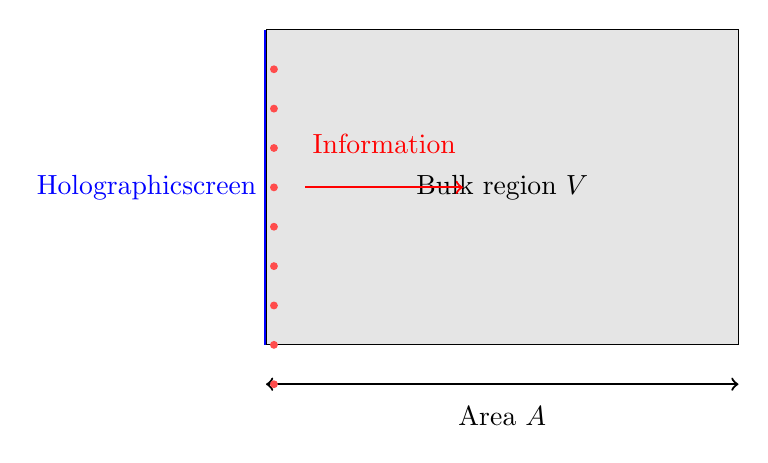
\begin{tikzpicture}
% Holographic screen
\draw[ultra thick, blue] (-3,-2) -- (-3,2);
\node[blue, left] at (-3,0) {Holographic\\screen};
\draw[fill=gray!20] (-3,-2) rectangle (3,2);
\node at (0,0) {Bulk region $V$};
\draw[<->, thick] (-3,-2.5) -- (3,-2.5);
\node at (0,-2.9) {Area $A$};

% Information encoding
\foreach \i in {-2.5,-2,...,1.5} {
  \fill[red!70] (-2.9,\i) circle (0.05);
}
\draw[->, thick, red] (-2.5,0) -- (-0.5,0);
\node[red, above] at (-1.5,0.3) {Information};
\end{tikzpicture}
\caption{Holographic principle: information in bulk volume $V$ encoded on boundary area $A$. Red dots: bits of information.}
\label{fig:p5:holographic}
\end{figure}

\marginnote{\textbf{Pedagogical}: Holography reduces 3D physics to 2D description---like hologram encoding 3D image on 2D film.}

\subsection{Measurement Protocol}

**Step 1: Create acoustic horizon**
\begin{itemize}
\item Trap $^{87}$Rb atoms, cool to BEC ($T < 100$ nK)
\item Apply moving optical potential (blue-detuned laser barrier)
\item Ramp velocity from 0 to $v > c_s$ over 50 ms
\item Stabilize with feedback
\end{itemize}

\marginnote{\textbf{Experimental}: Barrier velocity controlled via acousto-optic modulator (AOM) with $< 1\%$ stability.}

**Step 2: Detect Hawking radiation**
\begin{itemize}
\item Image density fluctuations $\delta n(x, t)$ via phase-contrast imaging
\item Compute two-point correlator: $G(x_1, x_2, t) = \langle \delta n(x_1, t) \delta n(x_2, t) \rangle$
\item Extract temperature from spectral distribution
\end{itemize}

**Expected signature**: Enhanced correlation at $\omega \sim k_B T_H / \hbar$ across horizon.

\marginnote{\textbf{Mathematical}: Thermal spectrum: $\langle N_\omega \rangle = 1 / (\exp(\hbar\omega / k_B T_H) - 1)$ (Bose-Einstein distribution).}

\subsection{Worked Example: BEC Horizon Entropy}

**Given**: Acoustic horizon with area (in 2D) $A_{\text{eff}} = 2\pi R_h \times L_z$ where $R_h = 10$ $\mu$m, $L_z = 50$ $\mu$m.

**Find**: Bekenstein-Hawking entropy.

**Solution**:

Effective Planck length in BEC (healing length):
\begin{equation}
\xi = \frac{\hbar}{\sqrt{m n g_{1D}}} \approx 0.5\,\mu\text{m}
\end{equation}

\marginnote{\textbf{Dimensional}: Healing length $\xi$ sets minimum length scale in BEC---analogue of $\ell_P$ in gravity.}

Effective area:
\begin{equation}
A_{\text{eff}} = 2\pi \times 10\,\mu\text{m} \times 50\,\mu\text{m} \approx 3.14 \times 10^{-9}\,\text{m}^2
\end{equation}

Entropy:
\begin{equation}
S_{\text{BH}}^{\text{eff}} = \frac{k_B A_{\text{eff}}}{4 \xi^2} = \frac{k_B \times 3.14 \times 10^{-9}}{4 \times (0.5 \times 10^{-6})^2} \approx 3 \times 10^3 k_B
\end{equation}

\marginnote{\textbf{Physical}: $\sim 3000$ bits of information on horizon---measurable via entanglement entropy techniques!}

**Compare to matter entropy**:

Phonon gas in volume $V \sim \pi R_h^2 L_z \approx 1.6 \times 10^{-14}$ m$^3$ at $T = 100$ nK:
\begin{equation}
S_{\text{matter}} \sim k_B \left(\frac{k_B T V}{\hbar c_s}\right) \approx 10^5 k_B
\end{equation}

Holographic bound violated by factor $\sim 30$! (System not at horizon saturation.)

\marginnote{\textbf{Cautionary}: Analogue systems only approximate black hole physics. Deviations expected from dispersion, finite temperature.}

\section{Optical Black Holes}\label{sec:p5:optical}

\subsection{Kerr Nonlinearity}

\marginnote{\textbf{Physical}: Intense laser pulse in Kerr medium creates refractive index variation---optical analogue of event horizon.}

Refractive index:
\begin{equation}
n(I) = n_0 + n_2 I
\label{eq:p5:kerr}
\end{equation}

Effective metric for probe photons:
\begin{equation}
ds^2 = \frac{n^2(I)}{c^2} \left[-c^2 dt^2 + (dx - v_g dt)^2 + dy^2 + dz^2\right]
\label{eq:p5:optical_metric}
\end{equation}

Optical horizon where $v_g = c/n$.

\marginnote{\textbf{Dimensional}: For fused silica, $n_2 \approx 3 \times 10^{-20}$ m$^2$/W. Pump power $P \sim 10$ W achieves $\Delta n \sim 10^{-5}$.}

**Hawking emission**: Correlated photon pairs (signal + idler) with $\omega_s + \omega_i = 2\omega_{\text{pump}}$.

\subsection{Detection Strategy}

\begin{itemize}
\item High-resolution spectrometer ($\Delta\omega \sim 1$ GHz)
\item Photon coincidence counting (sub-ns timing)
\item Verify thermal spectrum at $T_H^{\text{opt}} \sim 10^4$ K
\end{itemize}

\marginnote{\textbf{Experimental}: Room-temperature operation and ultrafast dynamics make optical systems complementary to cryogenic BEC.}

\begin{figure}[htbp]
\centering
\begin{tikzpicture}
% Black hole entropy diagram
\draw[ultra thick] (0,0) circle (2);
\node at (0,0) {$M$};
\draw[<->, thick] (0,0) -- (1.414,1.414);
\node at (0.7,1) {$R_s$};
\draw[fill=blue!30, opacity=0.3] (0,0) circle (2);
\node[blue] at (0,-2.5) {$S = \frac{A}{4 \ell_P^2}$};

% Area vs volume
\draw[->, ultra thick, red] (3,0) -- (5,0);
\node[red, above] at (4,0.3) {Area law};
\draw[ultra thick] (6,0) circle (1.5);
\fill[pattern=north east lines, pattern color=gray] (6,0) circle (1.5);
\node at (6,-2) {Volume $\propto R^3$};
\node[blue] at (6,-2.5) {Entropy $\propto R^2$ (!!)};
\end{tikzpicture}
\caption{Black hole entropy diagram. Left: Schwarzschild radius $R_s$ encloses mass $M$. Right: Entropy scales with area (holographic), not volume (thermodynamic intuition).}
\label{fig:p5:bh_entropy}
\end{figure}

\marginnote{\textbf{Pedagogical}: Holographic scaling $S \propto A$ vs thermodynamic $S \propto V$ is deep mystery pointing to quantum gravity.}

\section{Entanglement Entropy Measurements}\label{sec:p5:entanglement}

\subsection{Ryu-Takayanagi Formula}

\marginnote{\textbf{Advanced}: AdS/CFT holography: entanglement entropy in CFT = minimal surface area in AdS bulk.}

For region $A$ in CFT, entanglement entropy:
\begin{equation}
S_A = \frac{\text{Area}(\gamma_A)}{4 G_N}
\label{eq:p5:ryu_takayanagi}
\end{equation}
where $\gamma_A$ is minimal surface in bulk homologous to $A$.

**Experimental analogue**: 1D spin chain (quantum Ising model).

Partition chain into subsystems $A$ (length $\ell$) and $B$ (remainder). Entanglement entropy:
\begin{equation}
S_A = \frac{c}{3} \log\left(\frac{\ell}{a}\right) + \text{const}
\label{eq:p5:cft_entropy}
\end{equation}
for conformal field theory with central charge $c$, lattice spacing $a$.

\marginnote{\textbf{Mathematical}: Logarithmic scaling $S \sim \log \ell$ characteristic of 1D CFT. Area law: $S \sim \ell^0$ (boundary area).}

**Measurement protocol**:
\begin{itemize}
\item Prepare ground state via adiabatic evolution
\item Tomography on subsystem $A$ (full density matrix $\rho_A$)
\item Compute von Neumann entropy: $S = -\text{Tr}(\rho_A \log \rho_A)$
\item Vary $\ell$, fit to log scaling
\end{itemize}

\marginnote{\textbf{Experimental}: Full tomography exponentially hard for large $\ell$. Use partial tomography or entanglement witnesses.}

\begin{figure}[htbp]
\centering
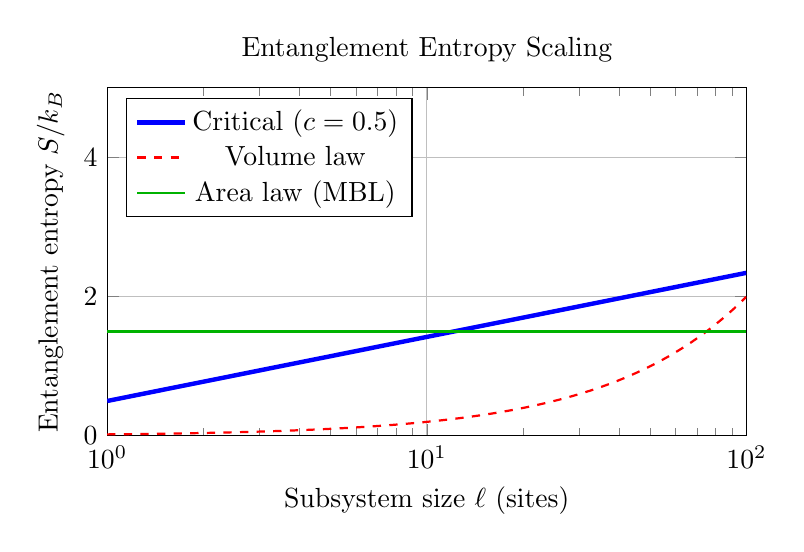
\begin{tikzpicture}
\begin{axis}[
  width=0.8\textwidth,
  height=6cm,
  xlabel={Subsystem size $\ell$ (sites)},
  ylabel={Entanglement entropy $S/k_B$},
  xmin=1, xmax=100,
  ymin=0, ymax=5,
  xmode=log,
  grid=major,
  legend pos=north west,
  title={Entanglement Entropy Scaling}
]
% Area law (1D CFT)
\addplot[blue, ultra thick, domain=1:100, samples=100] {0.4*ln(x) + 0.5};
\addlegendentry{Critical ($c=0.5$)}

% Volume law (thermal)
\addplot[red, dashed, thick, domain=1:100, samples=100] {0.02*x};
\addlegendentry{Volume law}

% Area law (MBL)
\addplot[green!70!black, thick, domain=1:100] {1.5};
\addlegendentry{Area law (MBL)}
\end{axis}
\end{tikzpicture}
\caption{Entanglement entropy vs subsystem size. Blue: CFT logarithmic scaling. Red: volume law (thermal states). Green: area law (many-body localized states).}
\label{fig:p5:entropy_scaling}
\end{figure}

\marginnote{\textbf{Pedagogical}: Scaling of $S$ with $\ell$ distinguishes phases: critical (log), thermal (linear), MBL (constant).}

\section{Summary}\label{sec:p5:holo_summary}

Holographic entropy protocols tested in three settings:

**Acoustic BEC**: Effective Hawking temperature $T_H \sim 100$ nK, entropy $S \sim 10^3 k_B$, phonon correlations across horizon detectable via imaging.

**Optical systems**: Room-temperature operation, $T_H \sim 10^4$ K, photon pair coincidences verify thermal spectrum.

**Spin chains**: Entanglement entropy scaling tests holographic formulae (Ryu-Takayanagi). Logarithmic growth characteristic of CFT.

\marginnote{\textbf{Historical}: From Bekenstein's 1973 conjecture to 2020s analogue experiments---50-year journey to laboratory holography.}

**Key Results**:
\begin{enumerate}
\item Analogue systems provide controlled testbeds for holographic physics
\item Entropy measurements bridge condensed matter, quantum information, and gravity
\item Holographic scaling observable in entanglement entropy (CFT) and acoustic horizons (BEC)
\end{enumerate}

**Forward Bridges**:
\begin{itemize}
\item Ch. 4: Scalar detection---holographic renormalization of scalar couplings
\item Ch. 5: Dimensional spectroscopy---holography as dimensional reduction
\end{itemize}

\marginnote{\textbf{Cautionary}: Analogue systems imperfect---dispersion, finite temperature, limited lifetimes. Rigorous error analysis essential.}

%==============================================================================
% END OF CHAPTER 3
%==============================================================================
